\chapter{Especificação}

\section{Componentes}
% TODO

\section{Stakeholders}
Com as funcionalidades e os módulos apresentados, podemos destacar os seguintes grupos dentre os potenciais consumidores:

\begin{itemize}
\item Pessoas que moram sozinhas e suas famílias, que podem estar interessadas em monitoramento;
\item Pessoas que desejam comodidade de controlar seus aparelhos numa interface única, pelo celular, e/ou conforto maior em casa;
\item Pessoas preocupadas com o consumo de água e energia elétrica.
\end{itemize}

Considerando o Censo de 2010 \cite{ibge}, podemos estimar grosseiramente as classes de consumidores para a cidade de São Paulo:

\begin{itemize}
\item Considerando que 1/10 da população com mais de 60 anos more sozinha e que 1/4 deles adquiriria o produto, temos uma estimativa de 33 mil consumidores. Como essa população está envelhecendo em taxas cada vez maiores (8,96\% em 2000 contra 13,6\% em 2016) \cite{bibliotecaVirtual}, a tendência é que essa classe aumente;
\item Considerando que 1/100 dos domicílios ocupados tenha uma pessoa com esse perfil, temos uma estimativa de 35 mil consumidores em potencial;
\item Considerando que cerca de 70\% das residências reduziram o consumo com campanhas de redução de uso de água em 2015 \cite{g1}, supondo que 5\% ficariam preocupados/interessados ao nível de se tornarem consumidores, temos uma estimativa de 71 mil consumidores em potencial.
\end{itemize}

\section{Requisitos}

\subsection{Requisitos Funcionais}
\begin{itemize}
\item O sistema deve permitir o monitoramento de aparelhos do dia a dia, dentro de uma residência, em módulos independentes;
\item O sistema deve ser capaz de enviar notificações aos usuários, seja por meio de um serviço no cliente utilizado pelo usuário (web ou aplicativo \textit{mobile});
\item O sistema deve poder ser personalizável pelo usuário, o qual pode adquirir novos módulos ou retirar algum já existente;
\item O sistema deve ser capaz de aprender a respeito de cada usuário, utilizando conceitos de Machine Learning. O aprendizado de máquina é responsável por detectar padrões no comportamento do usuário, os quais podem ser utilizados para a segurança da casa. Assim, se o usuário, por padrão, chega em casa em uma janela de horário constante, e interage com certos módulos, caso haja uma atividade que não se enquadra no padrão, o comportamento pode ser considerado suspeito, e providências tomadas (como notificações para outros usuários, como alguém da família);
\item O sistema deve manter backup de dados do controlador local na nuvem;
\item O sistema deve permitir ao usuário o seu cadastro na plataforma, pela plataforma que melhor lhe convier;
\item O usuário poderá cadastrar sua casa na plataforma, podendo ter uma ou mais casas cadastradas;
\item O usuário poderá cadastrar os módulos dentro de uma casa, sendo que uma casa pode ter vários módulos, e cada módulo só poderá existir em uma casa;
\item O usuário pode efetuar as operações de remoção e modificação nos seus módulos e casas;
% TODO rever item abaixo, acho que talvez essa funcao de reset nao tenha ficado muito claro. Tipo, o que ela faz, qual parte do sistema ela afeta, etc. Dado que nesse contexto, o "sistema" é tudo, ou seja, API, etc tb. E esse reset nao afetaria API. Entao acho que vale a reescrita desse requisito
\item O sistema deve possuir uma função de reset de fácil utilização.
\end{itemize}

\subsection{Requisitos Não-Funcionais}
O levantamento de requisitos não-funcionais foi realizado com base na norma ISO25010:2011 \cite{iso25010}.

\begin{itemize}
\item Os módulos que compõem o sistema dentro de uma residência devem ser independentes entre si, devendo obedecer a uma interface comum de integração com o core do projeto, para que seja facilitada a ampliação e a inserção de novos módulos, com outras funcionalidades. Haverá validação com o desligamento de um módulo e verificação do comportamento dos demais;
\item O sistema deve garantir segurança dos dados por meio de protocolo de comunicação seguro, tanto para o controle de acesso à API por usuários autenticados quanto para impedir que dados sejam interceptados em sua transmissão;
\item O banco de dados deve possuir acesso restrito e estar hospedado em servidor de alta segurança;
% TODO como assim "em menos de 10 minutos"? podemos mover para uma seção específica do módulo de acesso
\item O sistema deve ser robusto, de modo a continuar operando, mesmo com menor nível de funcionalidades, quando da ocorrência de falhas na comunicação com a nuvem (indisponibilidade parcial devido a problemas com os servidores remotos, ou total com perda da conexão com a Internet) ou falhas na rede local (indisponibilidade da conexão com a rede local). Também deve se recuperar em caso de travamento total do módulo e continuar funcionando em caso de DoS Local. Para validação, haverão testes de indisponibilidade de servidor, conexão com a internet, rede local e DoS local, e observação da continuidade de serviço de atuação na iluminação da casa e abertura do portão em menos de 10 minutos;
% TODO era bom falar algo sobre os dois itens abaixo (tipo, se a gente fez algo pra tentar seguir essa meta)
\item O sistema deve apresentar disponibilidade de 99,9\% - cerca de 8 horas de indisponibilidade por ano -, não levando em consideração problemas com a conexão de internet da residência;
\item O sistema deve ser escalável a até 10 mil usuários, sem perdas de desempenho consideráveis, ou aumento na latência para as requisições serem atendidas;
\item O sistema deve possuir instalação intuitiva e simplificada.
\end{itemize}

\subsection{Requisitos por Nível de Conectividade}

% TODO melhorar legibilidade da tabela
\begin{figure}[H]
	\centering
	\caption{Tabela de requisitos por nível de conectividade}
  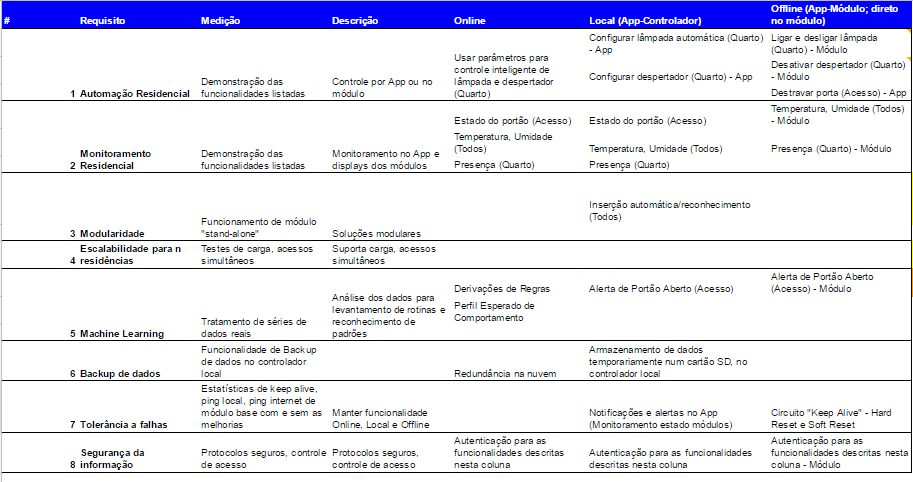
\includegraphics[width=0.95\textwidth]{tabelaRequisitos}
\label{fig:tabelaRequisitos}
\end{figure}
